% A hand-drawn, entirely vector TikZ interpretation of IMG_4707.jpeg.
% Self-contained: no external pictures, fonts, data files, or shell escape.
% Compile with: pdflatex IMG_4707.tex
\documentclass[tikz,border=0pt]{standalone}
\usepackage{tikz}
\usetikzlibrary{calc}

% Paint palette, sampled visually from the reference.
\definecolor{skyTop}{HTML}{586C96}
\definecolor{skyBlue}{HTML}{2C6396}
\definecolor{skyDeep}{HTML}{2B527F}
\definecolor{haze}{HTML}{887587}
\definecolor{warmHaze}{HTML}{D28759}
\definecolor{sunOrange}{HTML}{FF792C}
\definecolor{sunFire}{HTML}{FF5422}
\definecolor{sunCoral}{HTML}{FB7161}
\definecolor{sunGold}{HTML}{FFC66D}
\definecolor{starCream}{HTML}{F3EBA7}
\definecolor{starGold}{HTML}{DDD52B}
\definecolor{hairGold}{HTML}{FFAF13}
\definecolor{hairLight}{HTML}{FFE078}
\definecolor{hairOrange}{HTML}{FF8B05}
\definecolor{hairRed}{HTML}{FF5F13}
\definecolor{hairShade}{HTML}{D57520}
\definecolor{scarfRed}{HTML}{EE2319}
\definecolor{scarfLight}{HTML}{FF4422}
\definecolor{scarfDark}{HTML}{C91619}
\definecolor{coat}{HTML}{426231}
\definecolor{coatLight}{HTML}{72833F}
\definecolor{coatMid}{HTML}{577536}
\definecolor{coatDark}{HTML}{294B37}
\definecolor{coatDeep}{HTML}{293F36}
\definecolor{belt}{HTML}{74332F}
\definecolor{beltLight}{HTML}{A44C4A}
\definecolor{boot}{HTML}{7B2C27}
\definecolor{skin}{HTML}{F3D76A}
\definecolor{rim}{HTML}{F8DC99}
\definecolor{planetRust}{HTML}{8D3D2D}
\definecolor{planetRed}{HTML}{C44329}
\definecolor{planetDark}{HTML}{272C28}
\definecolor{planetBlue}{HTML}{254A64}
\definecolor{planetLight}{HTML}{355875}
\definecolor{roseDark}{HTML}{9F161C}
\definecolor{rose}{HTML}{C62125}
\definecolor{roseLight}{HTML}{DF3F37}
\definecolor{stem}{HTML}{283B28}
\definecolor{glass}{HTML}{FCE4C0}

% Shared silhouettes keep the painted details inside the subject.
\def\hairshape{(5.11,8.08)
 .. controls (4.94,8.33) and (4.90,8.62) .. (4.98,8.87)
 .. controls (4.89,8.73) and (4.80,8.58) .. (4.77,8.58)
 .. controls (4.78,8.87) and (4.91,9.22) .. (5.03,9.39)
 -- (4.73,9.31) -- (4.89,9.54) -- (5.22,9.67)
 .. controls (5.10,9.75) and (5.09,9.85) .. (5.14,10.00)
 -- (5.30,9.91) -- (5.27,10.14) -- (5.47,10.03)
 -- (5.48,10.20) -- (5.67,10.13) -- (5.74,10.29)
 -- (5.86,10.20) -- (6.01,10.25) -- (6.10,10.07)
 -- (6.21,10.28) -- (6.29,10.09) -- (6.51,10.16)
 -- (6.43,9.94) -- (6.67,10.00) -- (6.64,9.83)
 .. controls (6.73,9.84) and (6.78,9.82) .. (6.77,9.74)
 -- (6.66,9.60)
 .. controls (6.88,9.49) and (7.06,9.22) .. (7.12,9.07)
 -- (6.99,9.12) -- (7.02,8.90) -- (6.94,8.98)
 .. controls (7.02,8.59) and (6.75,8.19) .. (6.46,8.03)
 .. controls (6.02,7.87) and (5.51,7.92) .. (5.11,8.08) -- cycle}
\def\coatshape{(5.50,7.82)
 .. controls (5.24,7.66) and (5.11,7.34) .. (4.99,7.03)
 .. controls (4.82,6.67) and (4.65,6.08) .. (4.54,5.61)
 .. controls (4.49,5.48) and (4.83,5.34) .. (5.21,5.36)
 .. controls (5.48,5.26) and (5.75,5.51) .. (6.05,5.52)
 .. controls (6.38,5.49) and (6.54,5.60) .. (6.82,5.47)
 .. controls (7.12,5.49) and (7.44,5.62) .. (7.75,5.84)
 .. controls (7.76,6.11) and (7.63,6.38) .. (7.48,6.60)
 .. controls (7.37,6.98) and (7.16,7.56) .. (6.87,7.87)
 .. controls (6.57,7.98) and (5.80,7.97) .. (5.50,7.82) -- cycle}
\def\trousershape{(5.21,5.62)
 .. controls (5.20,4.73) and (5.36,3.50) .. (5.67,3.01)
 .. controls (5.76,2.89) and (5.96,2.94) .. (6.06,3.11)
 -- (6.23,3.44)
 .. controls (6.30,3.23) and (6.43,3.02) .. (6.52,3.00)
 .. controls (6.62,2.94) and (6.77,3.02) .. (6.83,3.20)
 .. controls (7.15,3.64) and (7.18,4.80) .. (7.07,5.68)
 .. controls (6.53,5.83) and (5.70,5.86) .. (5.21,5.62) -- cycle}
\def\globeshape{(0,0.05)
 .. controls (2.16,1.49) and (4.23,2.46) .. (6.05,2.46)
 .. controls (7.89,2.48) and (10.38,1.70) .. (12,0.78)
 -- (12,0) -- (0,0) -- cycle}

\newcommand{\paintstar}[4]{%
 \begin{scope}[shift={(#1,#2)},scale=#3,rotate=#4]
  \fill[starCream,opacity=.08] (-.18,-.14)--(-.08,.02)--(-.15,.13)
   --(-.02,.12)--(.04,.24)--(.10,.08)--(.22,.01)--(.13,-.06)
   --(.15,-.18)--(.03,-.13)--(-.06,-.23)--(-.08,-.11)--cycle;
  \fill[starGold] (0,.17)--(.052,.054)--(.17,.019)--(.075,-.052)
   --(.095,-.16)--(-.005,-.096)--(-.12,-.15)--(-.075,-.036)
   --(-.17,.044)--(-.052,.066)--cycle;
  \draw[hairLight,line width=.65pt,opacity=.8]
   (-.07,-.13)--(-.025,.03)--(.05,.13) (.01,.015)--(.13,.005);
 \end{scope}}

\begin{document}
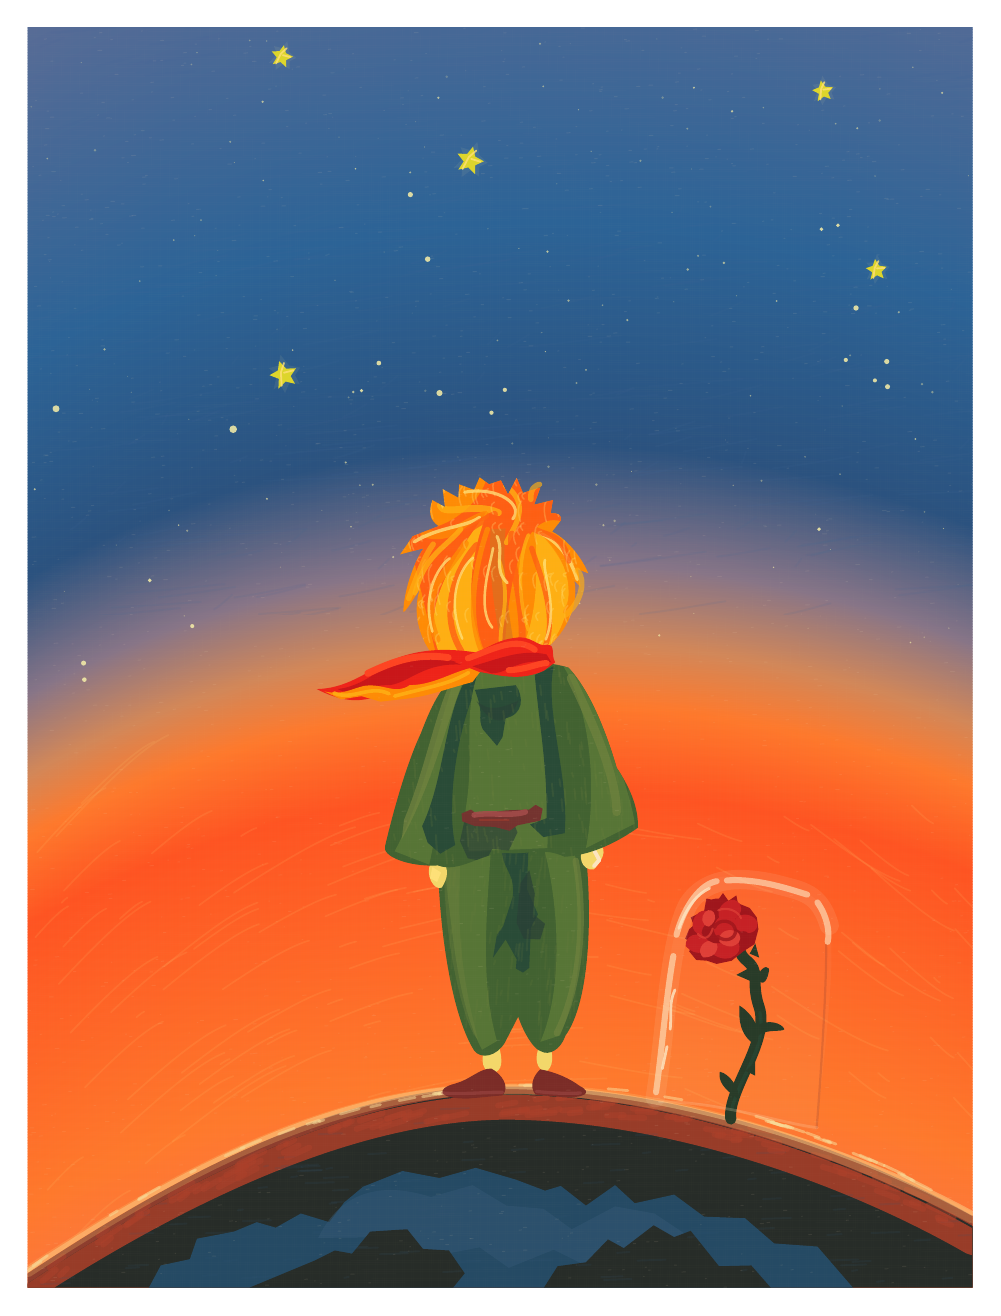
\begin{tikzpicture}[x=1cm,y=1cm,line cap=round,line join=round]
\path[use as bounding box] (0,0) rectangle (12,16);
\clip (0,0) rectangle (12,16);
\pgfmathsetseed{4707}

% Curved color bands reproduce the glow rising above the small planet.
% The bands overlap slightly so that the exported vector PDF has no seams.
\foreach \i in {-130,...,800}{
 \pgfmathsetmacro{\b}{\i/50}
 \ifdim\b pt<1pt
   \pgfmathtruncatemacro{\mix}{max(0,min(100,100*(\b+2.6)/3.6))}
   \colorlet{band}{sunOrange!\mix!sunCoral}
 \else\ifdim\b pt<4.6pt
   \pgfmathtruncatemacro{\mix}{100*(\b-1)/3.6}
   \colorlet{band}{sunFire!\mix!sunOrange}
 \else\ifdim\b pt<5.7pt
   \pgfmathtruncatemacro{\mix}{100*(\b-4.6)/1.1}
   \colorlet{band}{sunOrange!\mix!sunFire}
 \else\ifdim\b pt<6.5pt
   \pgfmathtruncatemacro{\mix}{100*(\b-5.7)/.8}
   \colorlet{band}{warmHaze!\mix!sunOrange}
 \else\ifdim\b pt<7.5pt
   \pgfmathtruncatemacro{\mix}{100*(\b-6.5)}
   \colorlet{band}{haze!\mix!warmHaze}
 \else\ifdim\b pt<9pt
   \pgfmathtruncatemacro{\mix}{100*(\b-7.5)/1.5}
   \colorlet{band}{skyDeep!\mix!haze}
 \else\ifdim\b pt<11.8pt
   \pgfmathtruncatemacro{\mix}{100*(\b-9)/2.8}
   \colorlet{band}{skyBlue!\mix!skyDeep}
 \else
   \pgfmathtruncatemacro{\mix}{max(0,min(100,100*(\b-11.8)/4.2))}
   \colorlet{band}{skyTop!\mix!skyBlue}
 \fi\fi\fi\fi\fi\fi\fi
 \fill[band] (0,\b)
  .. controls (3.7,{\b+2.08}) and (8.1,{\b+2.18}) .. (12,{\b+.65})
  -- (12,{\b+.68})
  .. controls (8.1,{\b+2.21}) and (3.7,{\b+2.11}) .. (0,{\b+.03})
  -- cycle;
}

% Dry-brush sky: long, faint, imperfect blue strokes.
\begin{scope}
 \clip (0,8.55) rectangle (12,16);
 \foreach \i in {1,...,310}{
  \pgfmathsetmacro{\px}{12*rnd}
  \pgfmathsetmacro{\py}{8.4+7.7*rnd}
  \pgfmathsetmacro{\len}{.05+1.3*rnd}
  \pgfmathsetmacro{\slope}{.04+.15*rnd}
  \draw[skyTop!55!skyBlue,opacity=.10,line width=.7pt]
   (\px,\py) .. controls ({\px+\len*.4},{\py+\slope*.3})
   and ({\px+\len*.8},{\py+\slope*.8}) .. ({\px+\len},{\py+\slope});
 }
\end{scope}

% Thin orange and peach brush arcs across the glowing lower sky.
\begin{scope}
 \clip (0,0) rectangle (12,8.9);
 \foreach \i in {1,...,170}{
  \pgfmathsetmacro{\px}{12*rnd}
  \pgfmathsetmacro{\py}{-.7+7*rnd}
  \pgfmathsetmacro{\len}{.06+1.5*rnd}
  \pgfmathsetmacro{\rise}{.16*(6-\px)*\len}
  \draw[sunGold,opacity=.13,line width=.6pt]
   (\px,\py) .. controls ({\px+\len*.5},{\py+\rise*.6})
   and ({\px+\len*.8},{\py+\rise*.9}) .. ({\px+\len},{\py+\rise});
 }
\end{scope}

% Scattered pinpricks; the five prominent hand-painted stars are explicit.
\foreach \i in {1,...,132}{
 \pgfmathsetmacro{\px}{12*rnd}
 \pgfmathsetmacro{\py}{8.1+7.85*rnd}
 \pgfmathsetmacro{\rr}{.005+.013*rnd}
 \pgfmathsetmacro{\alpha}{.22+.52*rnd}
 \fill[starCream,opacity=\alpha] (\px,\py) circle[radius=\rr];
}
\foreach \x/\y/\r in {
 .36/11.16/.044,2.61/10.90/.048,5.23/11.36/.039,
 4.46/11.74/.030,5.89/11.11/.027,6.06/11.40/.027,
 4.24/11.39/.022,4.86/13.88/.033,5.08/13.06/.035,
 10.52/12.44/.034,10.91/11.76/.033,10.76/11.52/.026,
 10.39/11.78/.027,10.92/11.44/.032,10.29/13.49/.024,
 10.08/13.44/.024,10.05/9.63/.025,.71/7.93/.032,
 .72/7.72/.029,2.09/8.40/.026,1.55/8.98/.025}
 \fill[starCream,opacity=.88] (\x,\y) circle[radius=\r];
\paintstar{3.23}{15.64}{.82}{-10}
\paintstar{10.10}{15.20}{.78}{12}
\paintstar{5.62}{14.32}{1.02}{-12}
\paintstar{10.78}{12.93}{.78}{8}
\paintstar{3.25}{11.60}{1.02}{19}

% The curved, rough-painted globe.
\fill[planetRust] (0,0.18)
 .. controls (2.16,1.61) and (4.15,2.57) .. (6.05,2.55)
 .. controls (8.05,2.58) and (10.34,1.84) .. (12,.91)
 --(12,0)--(0,0)--cycle;
\fill[planetDark] \globeshape;
\begin{scope}
 \clip \globeshape;
 \fill[planetBlue] (1.38,-.3)--(1.69,.28)--(2.06,.36)--(2.15,.62)
  --(2.62,.71)--(2.91,.83)--(3.15,.76)--(3.47,.94)--(3.83,.83)
  --(4.02,1.08)--(4.26,1.28)--(4.76,1.48)--(5.23,1.39)
  --(5.69,1.52)--(6.20,1.37)--(6.57,1.23)--(6.77,1.29)
  --(7.09,1.04)--(7.46,1.30)--(7.71,1.07)--(8.21,1.18)
  --(8.59,.90)--(9.11,.88)--(9.48,.56)--(10.03,.52)
  --(10.41,.08)--(10.74,-.3)--cycle;
 \fill[planetLight,opacity=.48] (3.69,.63)
  .. controls (4.00,1.27) and (4.55,1.33) .. (5.12,1.15)
  --(5.65,1.30)--(6.08,1.04)--(6.55,1.00)--(6.91,.74)
  --(7.46,1.03)--(7.96,.94)--(8.44,.62)--(8.67,.37)
  --(7.82,.46)--(7.17,.24)--(6.68,.48)--(6.11,.25)
  --(5.74,.51)--(5.01,.37)--(4.65,.64)--cycle;
 \fill[planetDark] (2.34,-.2)--(3.64,.34)--(3.90,.47)--(4.12,.43)
  --(4.35,.71)--(4.82,.74)--(5.02,.49)--(5.35,.47)--(5.55,.18)
  --(5.24,-.2)--cycle;
 \fill[planetDark] (6.43,-.2)--(6.73,.27)--(7.09,.32)--(7.37,.61)
  --(7.57,.50)--(7.95,.79)--(8.21,.64)--(8.42,.72)--(8.78,.27)
  --(9.19,.28)--(9.61,-.2)--cycle;
 \draw[planetRed,opacity=.72,line width=9pt]
  (0,-.03) .. controls (2.1,1.33) and (4.2,2.27) .. (6.05,2.29)
  .. controls (8.1,2.29) and (10.4,1.49) .. (12,.57);
 \foreach \i in {1,...,165}{
  \pgfmathsetmacro{\px}{12*rnd}
  \pgfmathsetmacro{\py}{2.6*rnd}
  \pgfmathsetmacro{\len}{.04+.33*rnd}
  \draw[planetLight,opacity=.12,line width=.7pt]
   (\px,\py)--({\px+\len},{\py+.012});
 }
\end{scope}
% Broken strokes give the painted crust an uneven edge.
\foreach \i in {1,...,88}{
 \pgfmathsetmacro{\px}{12*rnd}
 \pgfmathsetmacro{\py}{-.05464*\px*\px+.7157*\px+.07-.23*rnd}
 \pgfmathsetmacro{\len}{.07+.28*rnd}
 \pgfmathsetmacro{\rise}{(.7157-.10928*\px)*\len}
 \draw[planetRed!60!planetRust,opacity=.48,line width=2.1pt]
  (\px,\py)--({\px+\len},{\py+\rise+.025});
}
\draw[rim,opacity=.43,line width=1.7pt]
 (0,.22) .. controls (2.17,1.66) and (4.12,2.58) .. (6.05,2.55)
 .. controls (8.0,2.55) and (10.39,1.82) .. (12,.94);
\draw[sunGold,opacity=.25,line width=4pt]
 (0,.20) .. controls (2.20,1.64) and (4.08,2.54) .. (6.05,2.52)
 .. controls (8.07,2.55) and (10.29,1.78) .. (12,.88);
\foreach \i in {1,...,46}{
 \pgfmathsetmacro{\px}{11.85*rnd}
 \pgfmathsetmacro{\py}{-.05464*\px*\px+.7157*\px+.22+.025*(rnd-.5)}
 \pgfmathsetmacro{\len}{.055+.22*rnd}
 \pgfmathsetmacro{\rise}{(.7157-.10928*\px)*\len}
 \draw[rim,opacity=.52,line width=1pt]
  (\px,\py)--({\px+\len},{\py+\rise});
}

% Ankles and burgundy shoes are behind the trouser cuffs.
\fill[skin] (5.80,3.03)..controls(5.75,2.87)and(5.78,2.75)..(5.90,2.72)
 ..controls(6.04,2.75)and(6.03,2.88)..(5.99,3.05)--cycle;
\fill[skin] (6.50,3.07)..controls(6.43,2.91)and(6.46,2.77)..(6.58,2.74)
 ..controls(6.67,2.79)and(6.69,2.95)..(6.62,3.09)--cycle;
\fill[boot] (5.89,2.78)..controls(5.75,2.79)and(5.62,2.64)..(5.43,2.59)
 ..controls(5.18,2.53)and(5.20,2.39)..(5.60,2.40)
 --(6.03,2.44)..controls(6.13,2.55)and(6.02,2.71)..(5.89,2.78)--cycle;
\fill[boot] (6.51,2.77)..controls(6.70,2.74)and(6.89,2.65)..(7.01,2.56)
 ..controls(7.19,2.47)and(7.06,2.40)..(6.78,2.42)
 --(6.45,2.45)..controls(6.36,2.56)and(6.43,2.70)..(6.51,2.77)--cycle;
\draw[beltLight,opacity=.48,line width=1.2pt]
 (5.27,2.47)..controls(5.51,2.45)and(5.78,2.48)..(6.03,2.48)
 (6.46,2.49)..controls(6.64,2.47)and(6.85,2.46)..(7.02,2.47);

% Baggy green trousers with separate dark, irregular folds.
\fill[coat] \trousershape;
\begin{scope}
 \clip \trousershape;
 \fill[coatMid] (5.25,5.70)..controls(5.39,4.63)and(5.43,3.66)..(5.77,3.02)
 --(5.96,3.13)..controls(5.75,3.87)and(5.82,4.65)..(5.89,5.65)--cycle;
 \fill[coatLight,opacity=.35] (5.29,5.49)..controls(5.26,4.45)and(5.55,3.27)..(5.72,3.15)
 ..controls(5.40,4.34)and(5.50,4.97)..(5.49,5.54)--cycle;
 \fill[coatDark] (6.02,5.64)..controls(6.00,5.31)and(6.20,5.29)..(6.16,4.96)
 --(6.04,4.59)--(5.96,4.48)--(5.91,4.19)--(6.07,4.42)
 --(6.21,4.17)--(6.20,4.05)--(6.29,4.00)--(6.37,4.06)
 --(6.39,4.57)--(6.48,4.74)--(6.34,5.06)--(6.36,5.59)--cycle;
 \fill[coatDeep,opacity=.7] (6.37,5.30)--(6.44,5.00)--(6.42,4.74)
 --(6.57,4.62)--(6.51,4.42)--(6.30,4.43)--(6.21,4.63)--(6.25,5.12)--cycle;
 \fill[coatMid] (6.54,5.64)..controls(6.75,4.89)and(6.81,3.80)..(6.51,3.12)
 --(6.76,3.20)..controls(7.15,4.13)and(7.03,5.13)..(6.91,5.70)--cycle;
 \draw[coatLight,opacity=.62,line width=2.3pt]
  (6.96,5.42)..controls(7.10,4.62)and(7.00,3.78)..(6.72,3.23);
 \foreach \i in {1,...,110}{
  \pgfmathsetmacro{\px}{5.2+2*rnd}
  \pgfmathsetmacro{\py}{2.95+2.8*rnd}
  \pgfmathsetmacro{\len}{.03+.29*rnd}
  \draw[coatLight,opacity=.14,line width=.7pt]
   (\px,\py)--({\px+.017},{\py+\len});
 }
\end{scope}

% Small hands peek from the sleeves.
\fill[skin] (5.12,5.39)..controls(5.04,5.25)and(5.16,5.03)..(5.26,5.08)
 ..controls(5.34,5.21)and(5.35,5.31)..(5.27,5.42)--cycle;
\fill[hairLight] (5.14,5.34)--(5.11,5.20)--(5.20,5.15)--(5.25,5.27)--cycle;
\fill[skin] (7.09,5.65)..controls(6.96,5.48)and(7.04,5.29)..(7.19,5.31)
 ..controls(7.35,5.48)and(7.35,5.60)..(7.22,5.66)--cycle;
\draw[glass,line width=1.4pt] (7.20,5.54)--(7.26,5.43)--(7.19,5.35);

% The coat, with broad olive paint planes and deep blue-green folds.
\fill[coat] \coatshape;
\begin{scope}
 \clip \coatshape;
 \fill[coatMid] (5.50,7.95)..controls(5.25,7.31)and(5.07,6.30)..(4.66,5.54)
 --(5.10,5.37)..controls(5.29,6.23)and(5.35,7.36)..(5.72,7.91)--cycle;
 \fill[coatLight,opacity=.72] (5.36,7.67)..controls(5.16,7.23)and(5.03,6.53)..(4.78,5.94)
 --(4.75,5.69)..controls(5.19,6.51)and(5.32,7.20)..(5.56,7.78)--cycle;
 \fill[coatDark] (5.58,7.76)..controls(5.28,7.23)and(5.30,6.48)..(5.01,5.86)
 --(5.08,5.65)--(5.24,5.51)--(5.43,5.62)
 ..controls(5.30,6.20)and(5.49,7.30)..(5.79,7.80)--cycle;
 \fill[coatMid] (5.75,7.89)..controls(5.50,7.26)and(5.69,6.83)..(5.56,6.06)
 --(5.60,5.54)--(6.60,5.58)--(6.64,6.79)--(6.57,7.97)--cycle;
 \fill[coatDark] (5.68,7.59)..controls(5.81,7.24)and(5.70,7.27)..(5.78,7.09)
 --(5.96,6.88)--(6.03,6.99)--(6.07,7.23)
 ..controls(6.30,7.28)and(6.30,7.50)..(6.20,7.65)--cycle;
 \fill[coatDeep,opacity=.56] (5.70,7.45)..controls(5.87,7.14)and(6.09,7.10)..(6.23,7.45)
 ..controls(6.01,7.36)and(5.86,7.30)..(5.70,7.45)--cycle;
 \fill[coatDark] (6.44,7.78)..controls(6.49,7.21)and(6.60,6.62)..(6.59,5.96)
 --(6.38,5.88)--(6.55,5.72)--(6.82,5.77)
 ..controls(6.88,6.50)and(6.56,7.33)..(6.68,7.89)--cycle;
 \fill[coatMid] (6.77,7.94)..controls(7.16,7.37)and(7.23,6.30)..(7.09,5.58)
 --(7.71,5.89)..controls(7.65,6.36)and(7.16,7.65)..(6.92,7.98)--cycle;
 \draw[coatLight,opacity=.66,line width=3.1pt]
  (6.90,7.74)..controls(7.19,7.15)and(7.48,6.47)..(7.48,6.04);
 \fill[coatDeep,opacity=.65] (5.55,5.94)--(5.49,5.67)--(5.59,5.45)
 --(5.81,5.41)--(5.90,5.57)--(6.11,5.55)--(6.22,5.78)--(6.15,5.96)--cycle;
 \foreach \i in {1,...,165}{
  \pgfmathsetmacro{\px}{4.5+3.3*rnd}
  \pgfmathsetmacro{\py}{5.3+2.65*rnd}
  \pgfmathsetmacro{\len}{.025+.23*rnd}
  \draw[coatLight,opacity=.17,line width=.7pt]
   (\px,\py)--({\px-.015},{\py+\len});
 }
\end{scope}

% Short, worn burgundy belt across the back.
\fill[belt] (5.51,6.02)--(5.63,6.07)--(5.71,6.01)--(6.08,6.06)
 --(6.37,6.07)--(6.45,6.13)--(6.54,6.08)--(6.51,5.93)
 --(6.22,5.87)--(6.12,5.80)--(5.93,5.85)--(5.68,5.86)--(5.52,5.92)--cycle;
\draw[beltLight,line width=2.0pt,opacity=.87]
 (5.67,6.00)..controls(5.84,6.04)and(6.15,5.98)..(6.32,6.04);
\draw[scarfLight,opacity=.18,line width=.6pt] (5.74,5.94)--(6.11,5.94);

% Golden-orange hair; the silhouette and sweeping locks follow the painting.
\fill[hairOrange] \hairshape;
\begin{scope}
 \clip \hairshape;
 \fill[hairRed] (4.82,9.60)..controls(5.34,9.60)and(5.74,9.94)..(5.84,10.30)
 --(6.72,10.31)--(6.90,9.68)
 ..controls(6.36,9.98)and(6.12,9.21)..(6.06,8.13)
 --(5.22,7.90)--cycle;
 \fill[hairGold] (5.25,8.01)..controls(4.95,8.60)and(5.40,9.25)..(5.85,9.88)
 ..controls(5.51,9.04)and(5.63,8.46)..(5.82,7.97)--cycle;
 \fill[hairGold] (6.45,9.63)..controls(7.08,9.12)and(6.91,8.42)..(6.53,8.04)
 --(6.24,8.03)..controls(6.51,8.57)and(6.46,9.15)..(6.45,9.63)--cycle;
 \fill[hairShade,opacity=.65] (5.88,9.63)..controls(5.85,9.17)and(5.91,8.64)..(6.03,8.11)
 --(6.20,8.02)..controls(6.10,8.62)and(6.02,9.11)..(6.07,9.64)--cycle;
 \foreach \col/\w/\a/\b/\c/\d/\e/\f/\g/\h in {
  hairGold/4/5.24/9.93/5.28/9.79/5.69/9.98/5.98/9.84,
  hairLight/1.8/5.55/10.10/5.98/10.18/6.31/9.93/6.16/9.76,
  hairGold/3/6.07/10.18/6.40/9.94/6.18/9.67/6.08/9.46,
  hairOrange/5/5.04/9.58/5.37/9.49/5.49/9.69/5.81/9.81,
  hairLight/2/4.91/9.47/5.24/9.67/5.55/9.65/5.74/9.78,
  hairRed/4/5.18/9.18/5.48/9.58/5.63/9.66/5.93/9.82,
  hairGold/3/4.92/8.82/5.04/9.30/5.30/9.39/5.50/9.63,
  hairOrange/4/5.20/8.23/4.94/8.83/5.33/9.07/5.56/9.45,
  hairLight/1.5/5.14/8.33/4.99/8.86/5.26/9.20/5.36/9.26,
  hairRed/3.5/5.51/8.08/5.23/8.52/5.40/9.09/5.70/9.43,
  hairLight/1.4/5.52/8.24/5.30/8.76/5.51/9.17/5.66/9.27,
  hairOrange/3/5.77/8.07/5.58/8.50/5.66/9.10/5.84/9.63,
  hairLight/1.5/5.90/8.38/5.69/8.64/5.88/9.19/5.91/9.39,
  hairGold/2.2/6.02/8.10/5.95/8.43/6.17/8.64/5.99/9.23,
  hairLight/1.8/6.09/8.95/5.90/9.13/6.06/9.34/5.96/9.54,
  hairRed/4/6.26/8.01/6.35/8.60/6.11/9.17/6.15/9.57,
  hairGold/2/6.36/8.35/6.22/8.74/6.23/9.28/6.36/9.56,
  hairRed/3/6.55/8.10/6.76/8.49/6.48/9.13/6.40/9.39,
  hairLight/1.5/6.58/8.23/6.75/8.65/6.52/9.12/6.57/9.24,
  hairOrange/3.5/6.84/8.58/7.07/8.96/6.73/9.41/6.53/9.61,
  hairLight/2/6.98/8.99/6.86/9.36/6.68/9.49/6.53/9.57,
  hairRed/3.5/6.87/9.23/6.76/9.66/6.55/9.49/6.31/9.72}
  \pgfmathsetmacro{\lockwidth}{.62*\w}
  \draw[\col,line width=\lockwidth pt,opacity=.78]
   (\a,\b)..controls(\c,\d)and(\e,\f)..(\g,\h);
 \foreach \i in {1,...,125}{
  \pgfmathsetmacro{\px}{4.76+2.4*rnd}
  \pgfmathsetmacro{\py}{8.00+2.3*rnd}
  \pgfmathsetmacro{\len}{.04+.25*rnd}
  \draw[hairLight,opacity=.29,line width=.55pt]
   (\px,\py)..controls({\px-.035},{\py+\len*.4})
   and({\px-.04},{\py+\len*.8})..({\px+.015},{\py+\len});
 }
\end{scope}
% A few loose, luminous locks outside the main mass.
\draw[hairGold,line width=2pt,opacity=.66]
 (4.84,8.75)..controls(4.96,9.08)and(5.05,9.30)..(5.15,9.44)
 (6.83,8.54)..controls(7.04,8.71)and(7.09,8.99)..(6.98,9.11)
 (6.39,10.01)..controls(6.38,10.16)and(6.46,10.19)..(6.50,10.20);

% Scarf: windswept ribbon to the left, folded bright red around the neck.
\fill[scarfRed] (5.79,8.05)
 ..controls(5.39,8.12)and(5.04,8.12)..(4.71,8.00)
 ..controls(4.36,7.88)and(4.11,7.61)..(3.67,7.60)
 ..controls(3.97,7.45)and(4.18,7.42)..(4.45,7.51)
 ..controls(4.76,7.60)and(5.08,7.54)..(5.36,7.64)
 ..controls(5.63,7.73)and(5.69,7.91)..(5.94,7.91)--cycle;
\fill[scarfDark] (3.94,7.60)..controls(4.38,7.66)and(4.51,7.98)..(4.97,8.00)
 ..controls(5.17,8.01)and(5.39,7.98)..(5.52,7.91)
 ..controls(5.03,7.94)and(4.86,7.69)..(4.60,7.65)
 ..controls(4.31,7.66)and(4.11,7.49)..(3.94,7.60)--cycle;
\draw[scarfLight,line width=2.5pt]
 (4.32,7.80)..controls(4.64,7.95)and(4.92,8.06)..(5.34,8.00);
\fill[hairOrange] (3.77,7.57)..controls(4.00,7.52)and(4.10,7.60)..(4.27,7.64)
 ..controls(4.52,7.68)and(4.67,7.52)..(4.85,7.65)
 ..controls(5.21,7.65)and(5.48,7.89)..(5.80,7.89)
 --(5.65,7.69)..controls(5.24,7.58)and(5.07,7.50)..(4.74,7.47)
 --(4.48,7.44)--(4.24,7.51)--(3.98,7.47)--cycle;
\draw[hairGold,line width=1.3pt,opacity=.88]
 (3.89,7.55)..controls(4.12,7.45)and(4.35,7.66)..(4.59,7.54)
 (4.66,7.51)..controls(5.06,7.62)and(5.36,7.66)..(5.60,7.81);
\fill[scarfRed] (5.43,7.94)
 ..controls(5.74,8.05)and(5.94,8.23)..(6.19,8.25)
 ..controls(6.40,8.29)and(6.47,8.13)..(6.60,8.16)
 ..controls(6.71,8.17)and(6.64,8.03)..(6.70,7.94)
 --(6.55,7.83)..controls(6.25,7.70)and(6.01,7.77)..(5.73,7.82)--cycle;
\fill[scarfDark] (5.65,7.89)..controls(6.00,7.99)and(6.27,8.11)..(6.59,8.04)
 --(6.65,7.94)..controls(6.19,8.00)and(6.12,7.80)..(5.89,7.80)--cycle;
\draw[scarfLight,line width=2.2pt]
 (5.59,7.99)..controls(5.94,8.12)and(6.21,8.27)..(6.44,8.10)
 (6.11,7.84)..controls(6.35,7.85)and(6.48,7.93)..(6.59,7.93);

% Glass bell: a nearly invisible peach interior over the orange background.
\def\bellshape{(7.94,2.39)
 ..controls(8.06,3.04)and(8.08,4.24)..(8.30,4.73)
 ..controls(8.50,5.26)and(8.85,5.26)..(9.19,5.19)
 ..controls(9.61,5.12)and(10.03,5.07)..(10.16,4.71)
 ..controls(10.29,4.30)and(10.13,3.10)..(10.02,1.99)
 ..controls(9.48,2.11)and(8.54,2.39)..(7.94,2.39)--cycle}
\fill[glass,opacity=.055] \bellshape;

% Curving stem, sharp thorns, and sparse leaves inside the bell.
\draw[stem,line width=4.0pt]
 (8.93,2.14)..controls(8.88,2.50)and(9.43,3.13)..(9.29,3.56)
 ..controls(9.17,3.91)and(9.33,4.00)..(9.11,4.17)
 ..controls(8.99,4.28)and(9.07,4.44)..(8.94,4.52);
\draw[coatDark,opacity=.56,line width=1.2pt]
 (8.94,2.26)..controls(9.08,2.77)and(9.38,3.02)..(9.30,3.49);
\fill[stem] (9.25,3.07)..controls(9.04,3.21)and(9.03,3.39)..(9.04,3.58)
 ..controls(9.22,3.47)and(9.34,3.24)..(9.25,3.07)--cycle;
\fill[stem] (9.27,3.20)..controls(9.40,3.29)and(9.58,3.24)..(9.61,3.28)
 ..controls(9.58,3.36)and(9.40,3.41)..(9.27,3.33)--cycle;
\fill[stem] (9.03,2.39)..controls(8.83,2.53)and(8.77,2.62)..(8.79,2.74)
 ..controls(8.91,2.72)and(9.05,2.52)..(9.03,2.39)--cycle;
\fill[stem] (9.23,3.87)--(9.00,3.97)--(9.15,4.05)--cycle;
\fill[stem] (9.27,3.96)..controls(9.34,4.11)and(9.44,4.09)..(9.41,4.00)
 ..controls(9.39,3.88)and(9.31,3.80)..(9.27,3.96)--cycle;
\fill[stem] (9.17,4.24)--(9.24,4.37)--(9.29,4.19)--cycle;
\fill[stem] (9.12,2.75)--(9.24,2.87)--(9.24,2.69)--cycle;

% Deep red rose: overlapping irregular petals, never a geometric rosette.
\fill[roseDark] (8.49,4.16)--(8.40,4.27)--(8.46,4.36)--(8.35,4.43)
 --(8.40,4.55)--(8.46,4.60)--(8.42,4.70)--(8.59,4.78)
 --(8.62,4.94)--(8.76,4.91)--(8.83,5.01)--(8.90,4.91)
 --(9.00,4.98)--(9.02,4.88)--(9.17,4.82)--(9.26,4.70)
 --(9.28,4.55)--(9.23,4.36)--(9.09,4.27)--(8.94,4.15)
 --(8.75,4.11)--(8.63,4.15)--cycle;
\foreach \x/\y/\s/\rot/\c in {
 8.51/4.35/.78/-25/rose,8.59/4.63/.82/45/rose,
 8.75/4.82/.70/-15/roseDark,8.93/4.77/.83/20/rose,
 9.12/4.60/.79/-30/rose,9.07/4.38/.78/25/roseDark,
 8.88/4.29/.89/-8/rose,8.66/4.29/.64/20/roseLight,
 8.74/4.49/.92/-35/roseDark,8.87/4.58/.86/35/rose,
 8.92/4.42/.70/-18/roseLight,8.66/4.69/.54/55/roseLight}{
 \begin{scope}[shift={(\x,\y)},scale=\s,rotate=\rot]
  \fill[\c] (-.17,-.10)..controls(-.26,.06)and(-.09,.20)..(.06,.17)
   ..controls(.19,.15)and(.21,.00)..(.12,-.07)
   ..controls(.06,-.14)and(-.06,-.15)..(-.17,-.10)--cycle;
 \end{scope}
}
\draw[roseDark,line width=1.2pt,opacity=.80]
 (8.72,4.57)..controls(8.77,4.70)and(8.98,4.67)..(8.99,4.53)
 ..controls(8.99,4.42)and(8.85,4.38)..(8.76,4.46);
\draw[roseLight,line width=.75pt,opacity=.70]
 (8.51,4.49)..controls(8.61,4.39)and(8.67,4.46)..(8.70,4.56)
 (8.77,4.79)..controls(8.87,4.84)and(9.02,4.79)..(9.06,4.69);

% Broken cream reflections define the arch and left glass wall.
\draw[glass,opacity=.11,line width=7pt]
 (7.97,2.41)..controls(8.10,3.21)and(8.14,4.40)..(8.39,4.87)
 ..controls(8.65,5.26)and(9.13,5.20)..(9.47,5.13)
 ..controls(9.85,5.03)and(10.05,5.02)..(10.18,4.60);
\draw[glass,opacity=.61,line width=2.2pt]
 (7.98,2.48)..controls(8.05,2.98)and(8.11,3.71)..(8.20,4.21)
 (8.24,4.48)..controls(8.34,4.86)and(8.56,5.13)..(8.75,5.16)
 (8.88,5.17)..controls(9.28,5.20)and(9.70,5.05)..(9.90,4.99)
 (10.03,4.89)..controls(10.15,4.72)and(10.19,4.52)..(10.16,4.39);
\draw[glass,opacity=.83,line width=1pt]
 (8.06,2.78)--(8.12,3.06)
 (8.16,3.28)..controls(8.18,3.49)and(8.14,3.61)..(8.22,3.78)
 (8.27,4.56)..controls(8.38,4.86)and(8.51,5.00)..(8.66,5.07);
\draw[planetRust,opacity=.24,line width=.8pt]
 (10.14,4.35)..controls(10.15,3.88)and(10.07,2.63)..(10.02,2.03);
\draw[glass,opacity=.20,line width=1pt]
 (8.02,2.36)..controls(8.81,2.36)and(9.53,2.09)..(10.03,2.03);

% Fine canvas tooth, made from faint vector threads and flecks.
\foreach \i in {1,...,420}{
 \pgfmathsetmacro{\xx}{\i*12/421}
 \draw[glass,opacity=.012,line width=.20pt]
  (\xx,0)..controls({\xx-.035},5.6)and({\xx+.025},10.2)..(\xx,16);
}
\foreach \i in {1,...,560}{
 \pgfmathsetmacro{\yy}{\i*16/561}
 \draw[glass,opacity=.014,line width=.20pt]
  (0,\yy)..controls(4.1,{\yy+.019})and(8.0,{\yy-.018})..(12,\yy);
}
\foreach \i in {1,...,1800}{
 \pgfmathsetmacro{\px}{12*rnd}
 \pgfmathsetmacro{\py}{16*rnd}
 \pgfmathsetmacro{\len}{.006+.045*rnd}
 \draw[glass,opacity=.085,line width=.35pt]
  (\px,\py)--({\px+\len},{\py+.002});
}
\end{tikzpicture}
\end{document}
